\documentclass{article}

\usepackage[letterpaper, portrait, margin=1.5in]{geometry}

\usepackage{fancyhdr}
\usepackage{ragged2e}
\usepackage{graphicx}
\usepackage{caption}
\usepackage{amsmath}
\usepackage{rotating}

\usepackage{listings}
\usepackage{color}

\definecolor{dkgreen}{rgb}{0,0.6,0}
\definecolor{gray}{rgb}{0.5,0.5,0.5}
\definecolor{mauve}{rgb}{0.58,0,0.82}

\lstset{frame=tb,
  language=Java,
  aboveskip=3mm,
  belowskip=3mm,
  showstringspaces=false,
  columns=flexible,
  basicstyle={\small\ttfamily},
  numbers=none,
  numberstyle=\tiny\color{gray},
  keywordstyle=\color{blue},
  commentstyle=\color{dkgreen},
  stringstyle=\color{mauve},
  breaklines=true,
  breakatwhitespace=true,
  tabsize=4
}

\setcounter{secnumdepth}{1}

\usepackage{chngcntr}
\counterwithin{figure}{section}

\renewcommand*{\thepage}{C\arabic{page}}

\pagestyle{fancy}
\lhead{ACME Robotics}
\chead{\#8367}
\rhead{\ifcontents Contents \else Week \thesection \fi}

\newif\ifcontents
\contentstrue

\makeatletter
\renewcommand{\@seccntformat}[1]{}
\makeatother
\begin{document}
\subsection{Attend the Burlingame Qualifier}
%! Go to the Burlingame qualifying tournament to compete.
This weekend, ACME Robotics attended the Burlingame qualifier. This was their first qualifier of the season and they were looking forward to seeing other robots teams had come up with, seeing how their robot performed and whether or not they would need to rethink their strategy for the next tournament.

The day began bright and early at 8 o'clock. The team arrived at the venue and set up their pit. Their pit had a poster board that Ben and Shawn had made, a huge collection of ACME wristbands and, of course, RedVines. ARES, ACME's sister team was also attending this tournament. This was their very first tournament and they were looking forward to seeing what competition was like. 

Next, the team prepared for their judging session. This was the first time Jon, Ashlin and Aidan had ever been to judging. Each team member had a talking point: Ben gave the intro, Jon and Aidan talked about outreach, Oren, Shawn and Ashlin discussed hardware and Emma and Kelly explained software. Judging went really well for them. The judges were engaged in their process and acknowledged their original and custom robot design, even if it wasn't entirely functional. They had really good questions and even gave the team time to talk about what they thought was unique about the team. 

Judging had put everyone in an excellent mood and Oren and Emma prepared for inspection. ACME notoriously never passes inspection for the first time, mainly due to not fitting inside of the 18. The team made it a goal for this tournament to pass both robot and field inspection the first time. Both went off without a hitch and qualifying matches began after opening ceremonies. 

As the team had such a complex robot design, they did not get it all done before the tournament. They had to rethink their strategy in order to even have a robot that could potentially score. Because of this, software didn't get the robot until that morning and they were rushing to have software to compete with. With matches about to start, the team had to make a quick decision: sit out the first match to have more time to work on the robot or put the robot on the field to see what would happen. The captains decided to allow more time to work on the robot and Emma went to the match as the team representative. This was a slight downer for the team, as it cost them a match, but they agree now that it was the right thing to do. 

After several more matches, that the team did put the robot on the field for, judges started to come around. Three groups of judges talked to the team: control, design and connect. Each of the captains had a chance to talk to the judges more about their subteam and all three of the interviews went off without a hitch. 

At the end of qualification matches, ACME placed 20th and ARES 18th. ACME was super proud of ARES and their performance. A few team members had to go home to work on homework, but a few stayed to watch finals and for the awards ceremony. The team was nominated for two awards, Control and Connect, which they were very proud of. However the best surprise came when the final awards winner was announced. ACME had won the Inspire Award! The team had never qualified for the Northern California Regionals at the first tournament and were very honored and relieved. This meant that the team only had to worry about making the robot as perfect as possible and not have to stress about qualifying. Everyone was super excited to win this award and could not have been happier. The team is looking forward to the next competitions to come!

\subsection{Post Match Retrospective}
%! Have a retrospective with the team for the Burlingame tournament.
After such an eventful tournament for ACME, the team had a retrospective to assess their performance. This gives ACME a good sense of what they did wrong, what they did right, and how they can improve for next time. Helping ACME to decide exactly where they want to go next with the robot and the team as a whole, and how to get there. Some of the things the team thought they did well was judging, the business notebook, and the drivetrain was very solid. Some things they thought didn’t go well was the robot wasn’t nearly as functional as it needed to be, keeping up with EN entries, and, perhaps most importantly, they didn’t where tutus! After writing down and sorting all the reflections of the various team members; the team discussed them further and created goals for the upcoming Intel tournament. Goals are essential because they give the team something to work towards as well as keeping them focused on the important tasks. Some of the goals the team is now working towards are to deploy from, and re-latch to, the lander, create a hard deadline for EN entries, and finish the scouting app to streamline scouting. Overall the team was happy with how the retrospective went and excited to move forward and improve. 

\begin{figure}
    \centering
    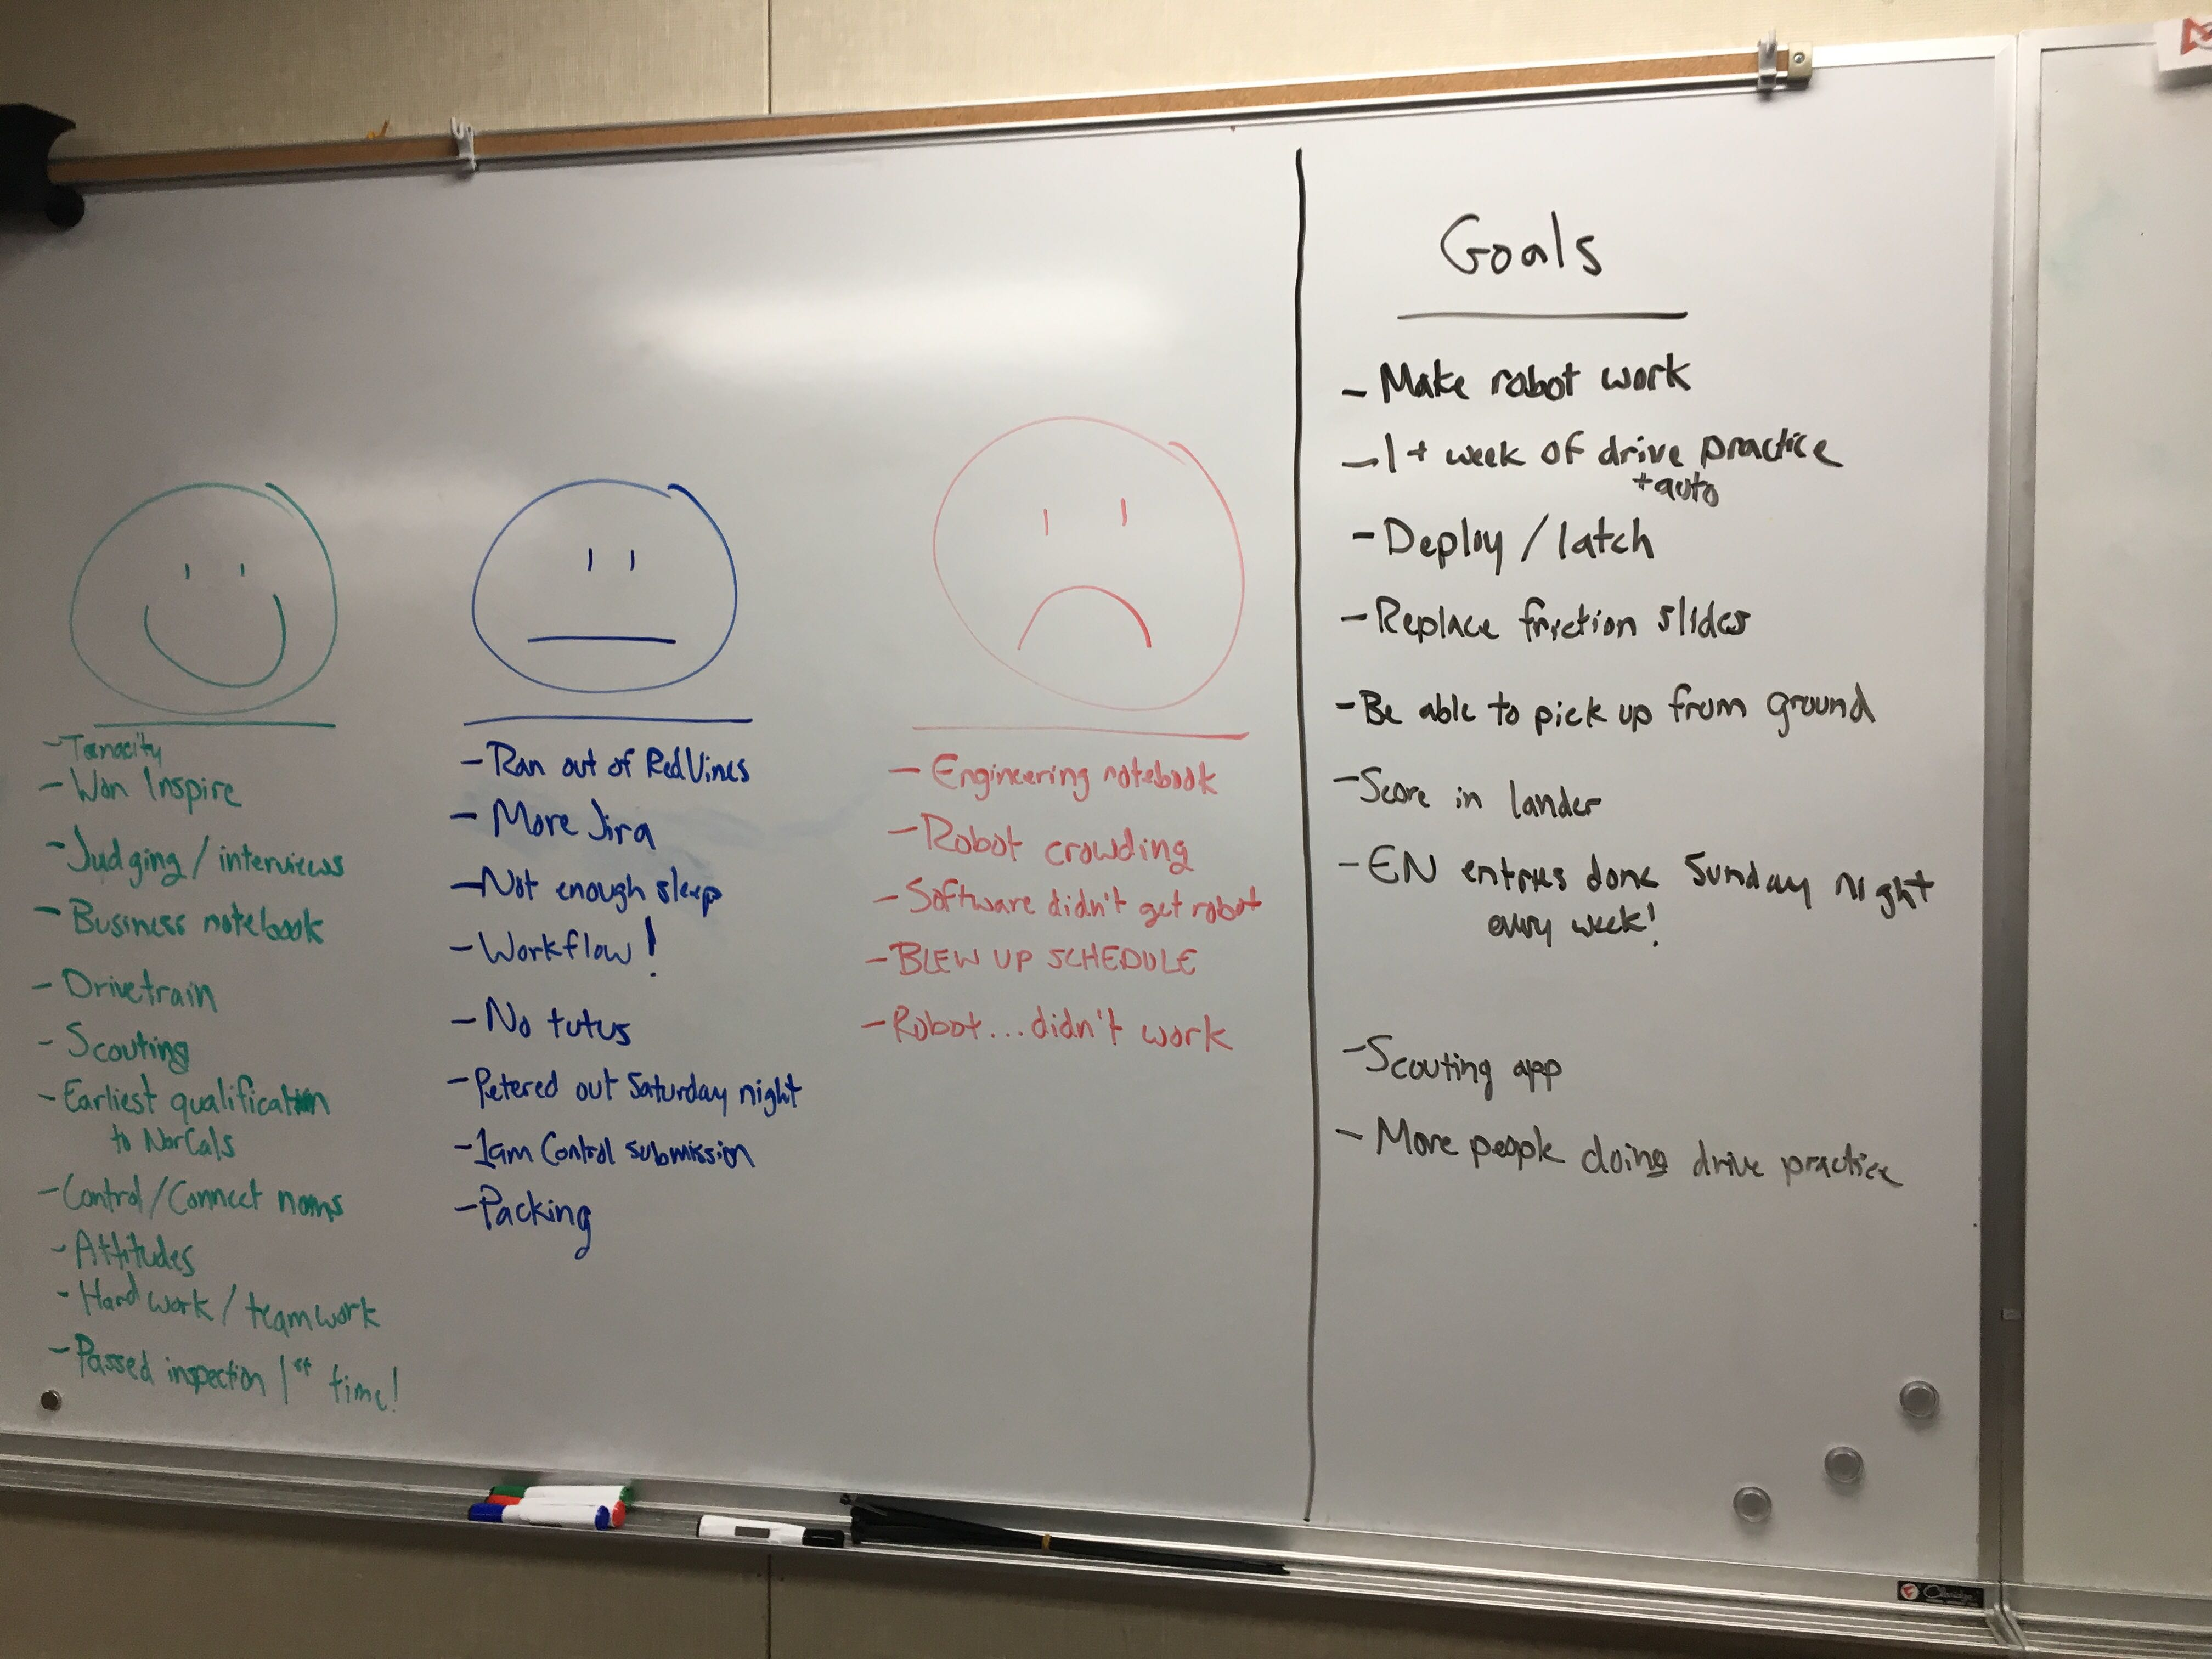
\includegraphics[width=.6 \textwidth]{12_11-19/images/retrospective.JPG}
    \caption{Burlingame Retrospective}
    \label{fig:retrospective}
\end{figure}

\end{document}